\documentclass[10pt]{beamer}
\usetheme{CambridgeUS}
\usepackage[utf8]{inputenc}
\usepackage[spanish]{babel}
\usepackage{amsmath}
\usepackage{amsfonts}
\usepackage{amssymb}
\usepackage{graphicx}
\usepackage{ragged2e}
\usepackage{multicol}
\usepackage{multirow, array}
\author{Kevin García - Alejandro Vargas}
\title{Gráfico de Control Multivariantes}
%\setbeamercovered{transparent} 
%\setbeamertemplate{navigation symbols}{} 
%\logo{} 
%\institute{} 
%\date{} 
%\subject{} 
\justifying
\begin{document}

\begin{frame}[plain]
\maketitle
\end{frame}

\begin{frame}{Contenido}
\tableofcontents
\end{frame}

\section{Introducción}
\begin{frame}{Introducción}
Durante la Segunda Guerra Mundial la técnica estadística de gráficas de control univariadas fue la más utilizada a pesar de que los procesos y productos que se analizaban poseían en su gran mayoría dos o más características de calidad. Con el tiempo se dio la necesidad de aplicar herramientas estadísticas multivariadas para controlar en forma simultánea dos o más variables. Sin embargo, las técnicas multivariadas de control son técnicas muy complejas de utilizar, por los conceptos matemáticos que se manejan. Esta dificultad es superada posteriormente con el avance de los programas o software especializados en control estadístico de procesos, lo que originó un interés de las técnicas de control multivariado. 

~\\En esta exposición veremos la descripción y aplicación de los gráficos de control multivariados más utilizados en la práctica, por medio de los cuales se quiere conocer si un proceso está bajo control o si, por el contrario, éste se encuentra fuera de control y se deben tomar las medidas necesarias.
\end{frame}

\section{Antecedentes}
\begin{frame}{Antecedentes}
Para estudiar un poco cómo funcionan y en qué contextos se han aplicado los gráficos de control multivariantes se estudiaron tres artículos:
\begin{itemize}
\justifying
\item \textbf{Aplicación del control estadístico multivariado para medir la capacidad del proceso de fabricación de resortes de compresión en acero inoxidable}\textbf{\cite{A1}}, donde se realizó la carta de control multivariada para determinar los parámetros del proceso y luego se calculó el índice de capacidad multivariado para revisar cumplimiento. Los resultados permitieron evidenciar que el proceso en la fase inicial estaba en control y era capaz de cumplir las especificaciones, pero luego en la segunda fase se encontró un proceso con alta variabilidad y poca capacidad de cumplimiento.
\item  \textbf{Desarrollo de una aplicación para gráficos de control de procesos industriales}\textbf{\cite{A2}}, donde se crea una aplicación para el control estadístico de la calidad basado en un entorno gráfico cuyo motor de cálculo es el lenguaje R. El nombre de la librería es qcr que corresponden a las siglas Quality Control and Reability en la cual se implementan los gráficos de control de calidad más utilizados en este
campo.
\end{itemize}   
\end{frame}

\begin{frame}{Antecedentes}
Para estudiar un poco cómo funcionan y en qué contextos se han aplicado los gráficos de control multivariantes se estudiaron tres artículos:
\begin{itemize}
\justifying
\item \textbf{Gráficos de control no paramétricos basados en R-estadísticos con aplicación al caso multivariante}\textbf{\cite{A3}}, se propone la implementación en R de varios gráficos de control para procesos industriales. Se hace énfasis en los gráficos de control no paramétricos basados en rangos ordinales, tanto univariantes como multivariantes propuestos por Liu y realiza una comparación entre estos y los gráficos de control clásicos propuestos por Shewhart.
\end{itemize}    
\end{frame}

\section{Descripción de la metodología}
\begin{frame}{Metodología}
Las gráficas de control multivariadas son un tipo de gráfica de control de variables que muestra cómo las variables correlacionadas o dependientes influyen en forma conjunta en un proceso o resultado. Por ejemplo, puede utilizar una gráfica de control multivariada para investigar si la temperatura y la presión se encuentran bajo control en la producción de piezas plásticas moldeadas por inyección.

~\\Si los datos incluyen variables correlacionadas, entonces crear gráficas de control separadas para cada variable podría conducir a una interpretación errónea, debido a que las variables en conjunto afectan el proceso. Sin embargo, las gráficas de control multivariadas son más difíciles de interpretar que las gráficas de control clásicas de Shewhart. Por ejemplo, la escala de las gráficas de control multivariadas no está relacionada con la escala de ninguna de las variables. Además, las señales de fuera de control en gráficas de control multivariadas no revelan cuál variable (o combinación de variables) causó la señal.
\end{frame}

\begin{frame}{Metodología}
Los gráficos de control multivariantes más utilizados y los cuales se tratarán en esta exposición son:
\begin{itemize}
\item Gráfico de contorno y gráfico de control $\chi^2$
\item Gráfico $T^2$ o de Hotelling
\item Gráfico de control de varianza generalizada
\item Gráfico multivariante de promedios ponderados exponencialmente (MEWMA)
\item Gráfico multivariante de suma acumulativa (MCUSUM)
\end{itemize}
\end{frame}

\begin{frame}{Gráfico de contorno y gráfico de control $\chi^2$}
En la distribución normal multivariable, la densidad se describe mediante un elipsoide centrado en el vector medio con ejes en dirección a los vectores propios ($e$) de la matriz de covarianza, estableciendo $\mu$ como el origen y con la longitud
$$\pm c\sqrt{\lambda_j}e_j$$

~\\siendo 
$$(x-\mu)'\Sigma^{-1}(x-\mu)=c^2$$
~\\Si x se distribuye $N_{p}(\mu,\Sigma)$, entonces $(x-\mu)'\Sigma^{-1}(x-\mu)$ es $\chi^2_{\alpha,p}$

~\\Por lo tanto,

$$(x-\mu)'\Sigma^{-1}(x-\mu)\leq \chi^2_{\alpha,p}$$
\end{frame}

\begin{frame}{Gráfico de contorno y gráfico de control $\chi^2$}
\begin{figure}[h!]
  \centering
  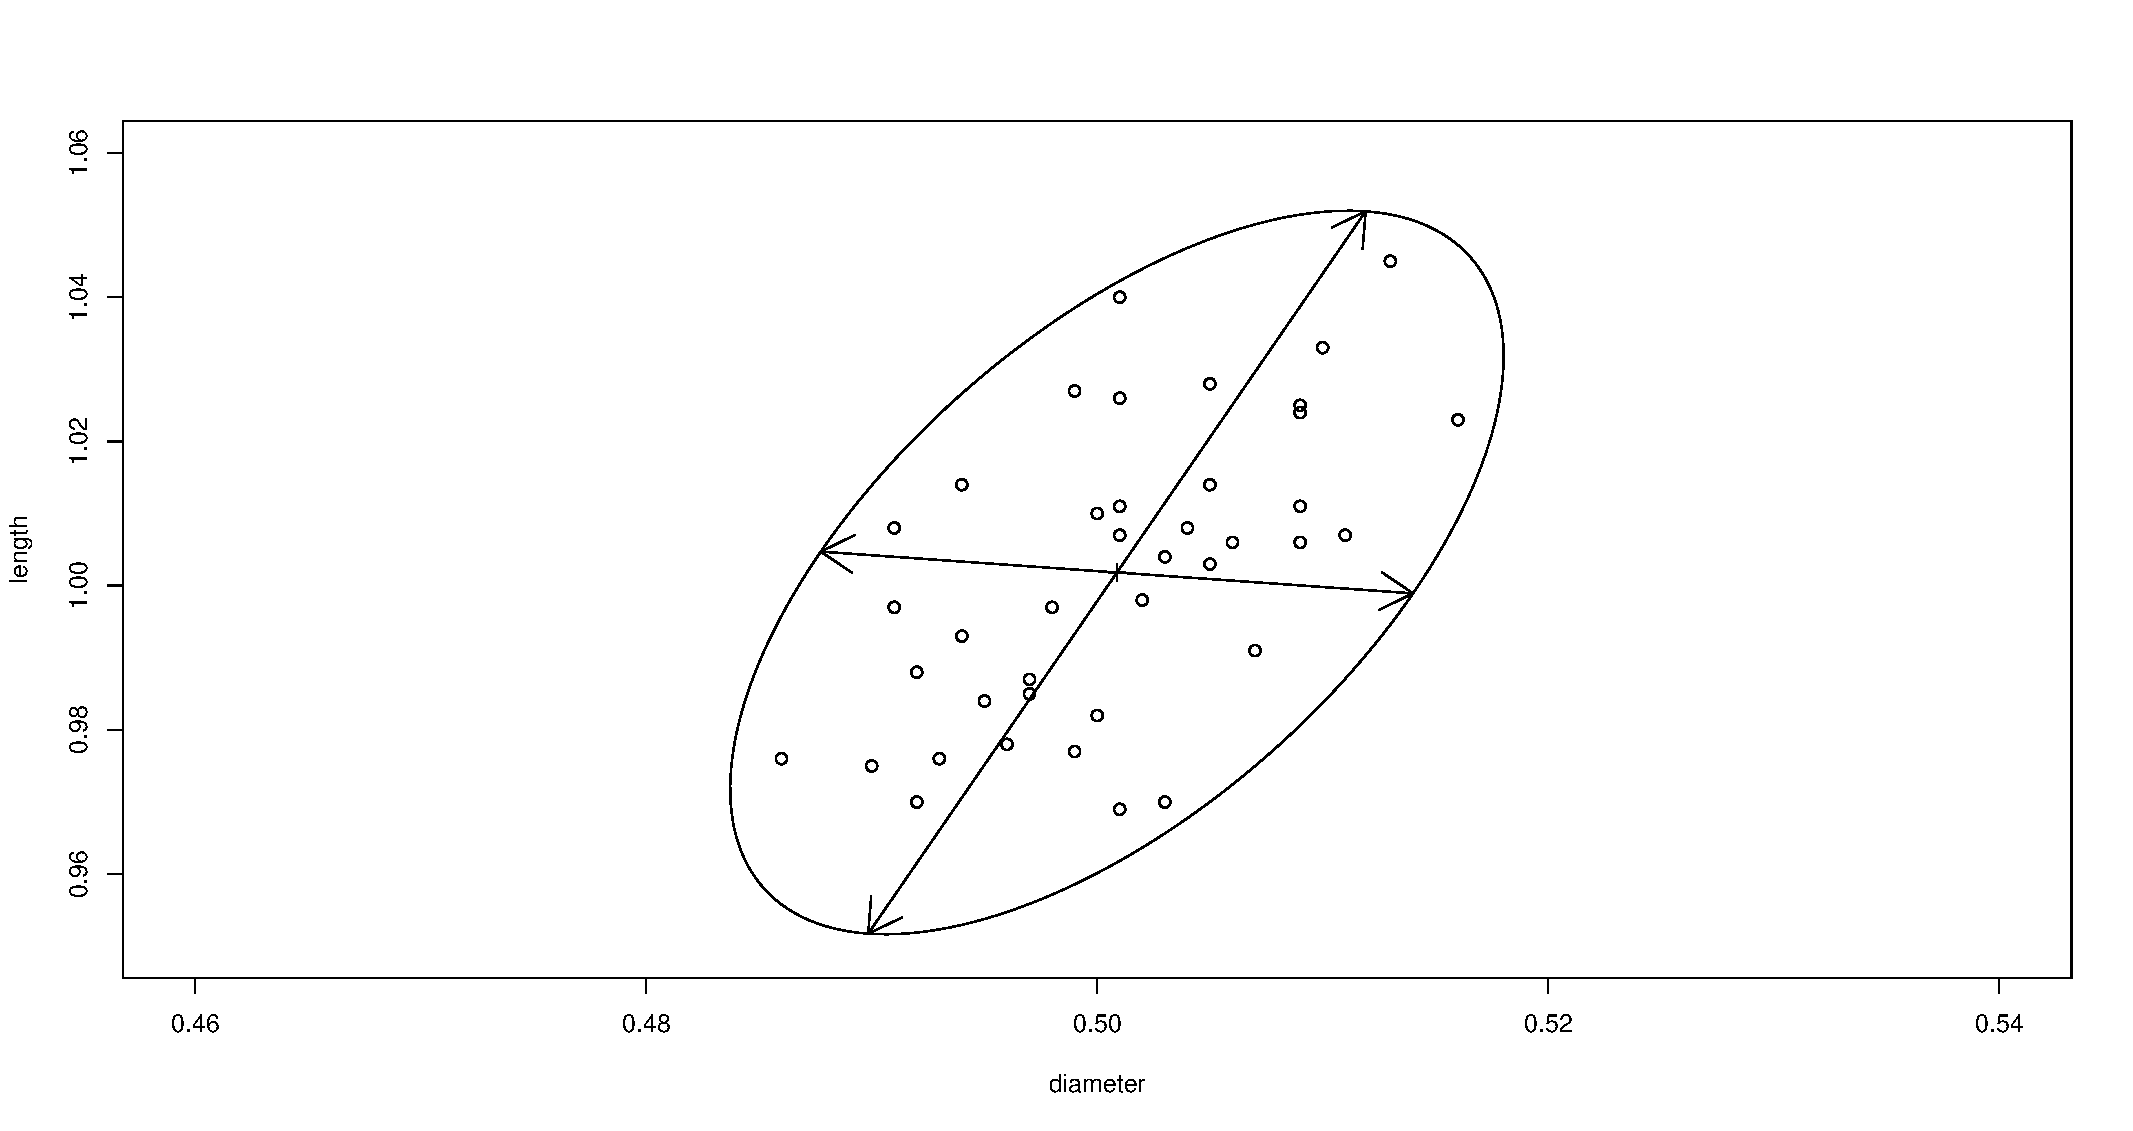
\includegraphics[scale=0.3]{FigurasUV/GC.pdf}
  \caption{Ejemplo gráfico de contorno}
\end{figure}
\end{frame}

\begin{frame}{Gráfico de contorno y gráfico de control $\chi^2$}
Al no obtener puntos fuera de la elipse, no hay evidencia de causas especiales; por lo tanto el proceso está en control. La dificultad para identificar los puntos más allá del elipsoide de confianza es uno de los principales inconvenientes de la herramienta. Otra desventaja es la complejidad para construir el elipsoide cuando $p> 2$, que se puede resolver utilizando el gráfico de control $\chi^2$ que se obtiene al trazar las estadísticas de la prueba:
$$n(x-\mu)'(\Sigma)^{-1}(x-\mu)= \chi^2_{\alpha,p}$$
Donde n es el tamaño de muestra y el límite de control superior:
$$UCL=\chi^2_{\alpha,p}$$
\end{frame}

\begin{frame}{Gráfico de contorno y gráfico de control $\chi^2$}
\begin{figure}[h!]
  \centering
  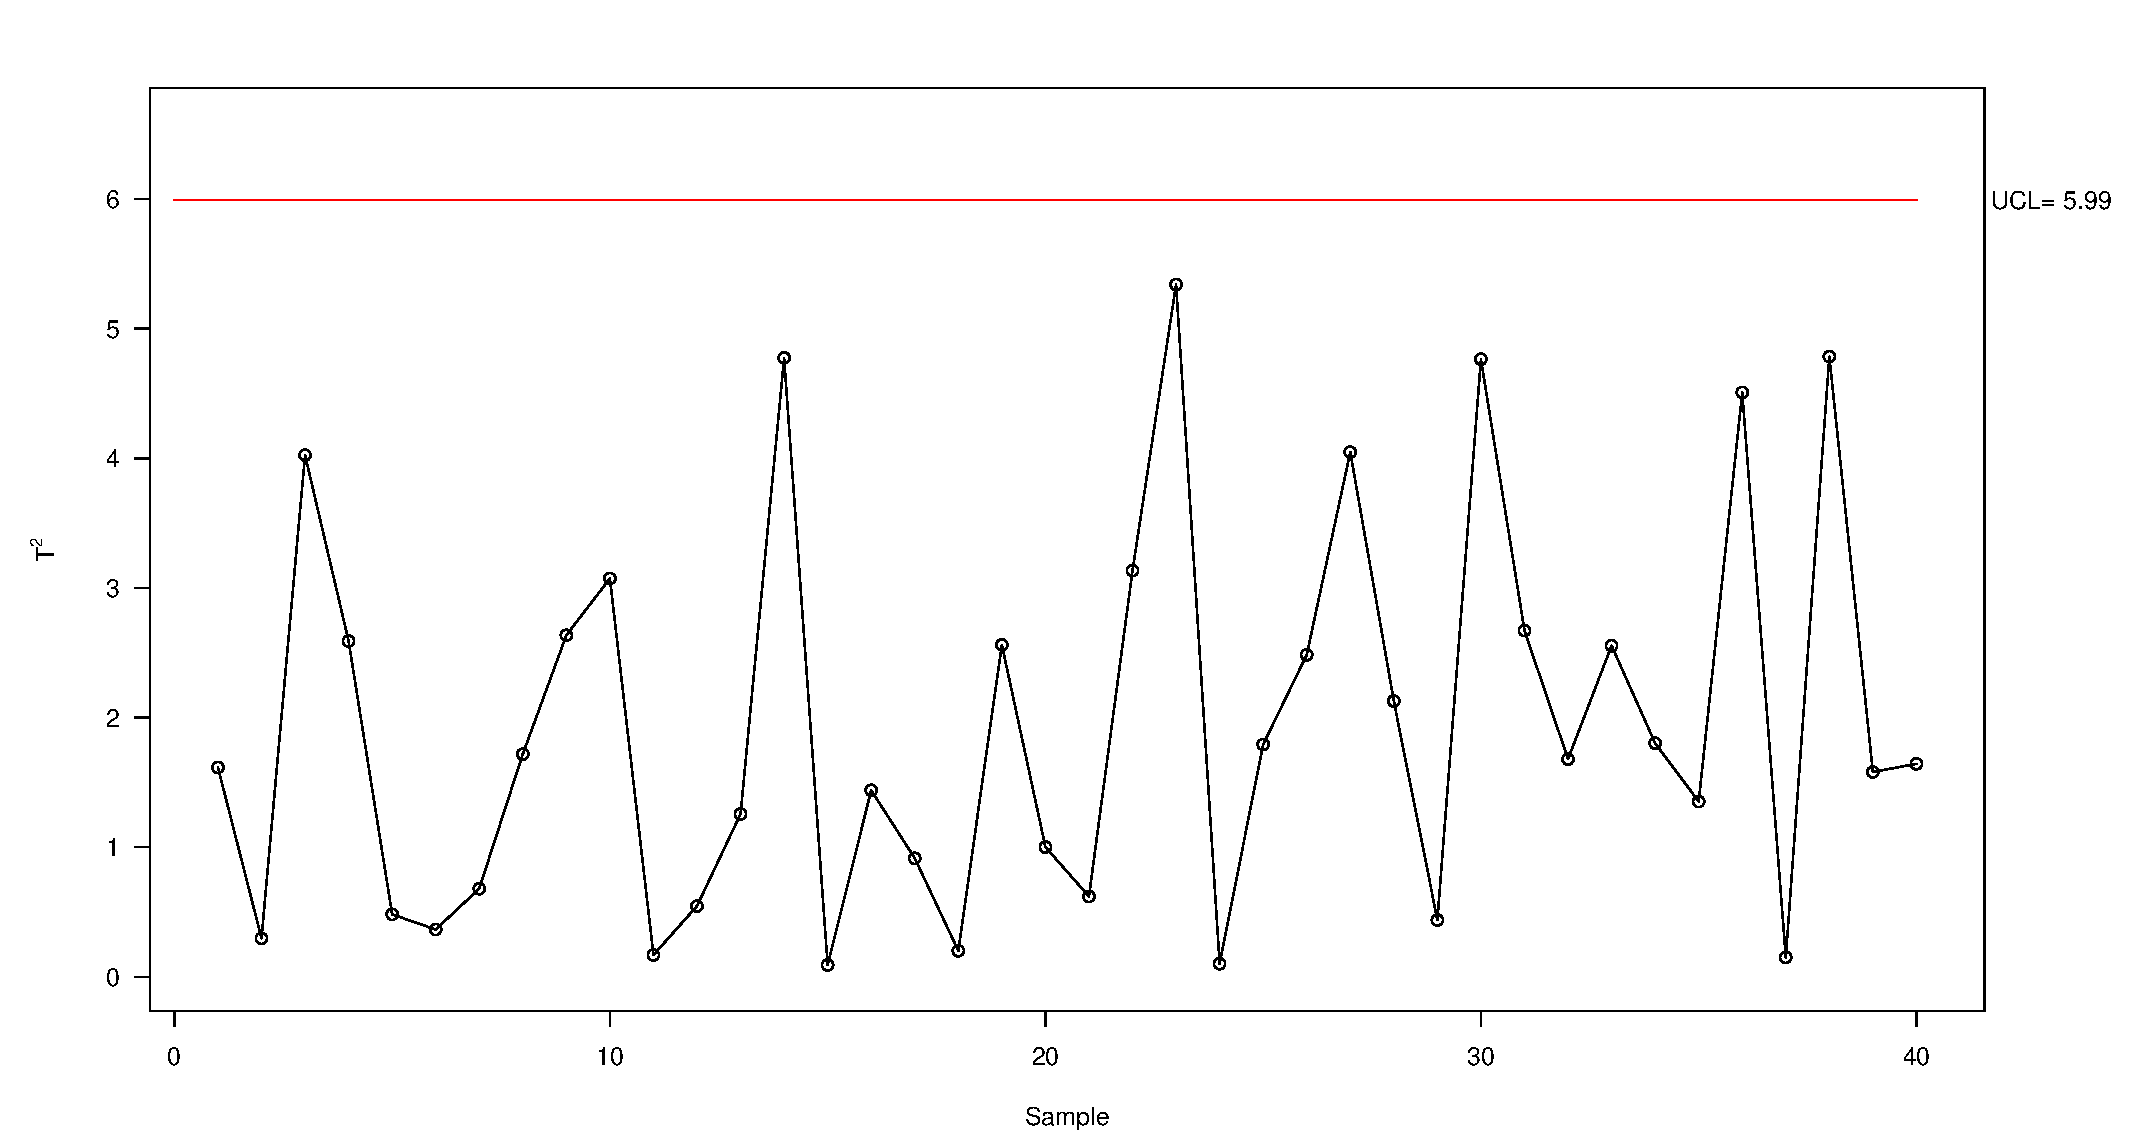
\includegraphics[scale=0.3]{FigurasUV/GChi2.pdf}
  \caption{Ejemplo gráfico de control $\chi^2$}
\end{figure}

Mostrando resultados iguales al control elipsoide. Una ventaja de este gráfico es que permite ver la evolución de las muestras a lo largo del tiempo.
\end{frame}

\begin{frame}{Gráfico $T^2$}
El procedimiento de Hotelling (1947) se ha convertido, sin duda, en el más aplicado en el control de procesos multivariado y es el análogo multivariado del gráfico de control de Shewhart. Por esa razón, también se conoce como gráfico de control Shewhart multivariado. En la práctica, los parámetros $\mu$ y $\Sigma$ son desconocidos y, por lo tanto, deben estimarse a través de los estimadores no sesgados $\bar{x}$ y $S$. En base a la generalización multivariable del estadístico $t$ a partir de la teoría normal univariada:
$$t=\frac{\bar{x}-\mu}{S/\sqrt{n}}$$
$$t^2=\frac{(\bar{x}-\mu)^2}{S^2/n}=n(\bar{x}-\mu)(S^2)^{-1}(\bar{x}-\mu)$$
por lo que la generalización resulta en
$$T^2=n(\bar{X}-\bar{\bar{X}})'(S)^{-1}(\bar{X}-\bar{\bar{X}})$$

~\\con $\bar{X}$ y $S$ vector de medias y matriz de covarianza, respectivamente.
\end{frame}

\begin{frame}{Gráfico $T^2$}
El estadistico $T^2$ sigue una distribución $F$ con $p$ y $(mn-m-p+1)$ grados de libertad. Por lo tanto, para establecer el control en la Fase I, los resultados de UCL en
$$UCL=\frac{p(m-1)(n-1)}{mn-m-p+1}F_{\alpha,p,mn-m-p+1}$$
Mientras para monitorear futuras observaciones (Fase II), el límite está dado por 
$$UCL=\frac{p(m+1)(n-1)}{mn-m-p+1}F_{\alpha,p,mn-m-p+1}$$
Aquí, el número de muestras ($m$) se refiere a las muestras preliminares tomadas para establecer el estado de control (Fase I). Este gráfico carece de límites de control inferiores (LCL) de manera análoga al gráfico $\chi^2$.

Este gráfico se emplea en estudios multivariados introductorios y tiene un buen desempeño en la detección de grandes cambios en la media. Según Lowry y Montgomery (1995), la aplicación de este gráfico requiere varias características de calidad entre 2 y 10, y toma más de 20 muestras (a menudo más de 50) de tamaño 2, 3 o 10. Estos valores a veces están limitados por la misma naturaleza del problema. 
\end{frame}

\begin{frame}{Gráfico $T^2$}
\begin{figure}[h!]
  \centering
  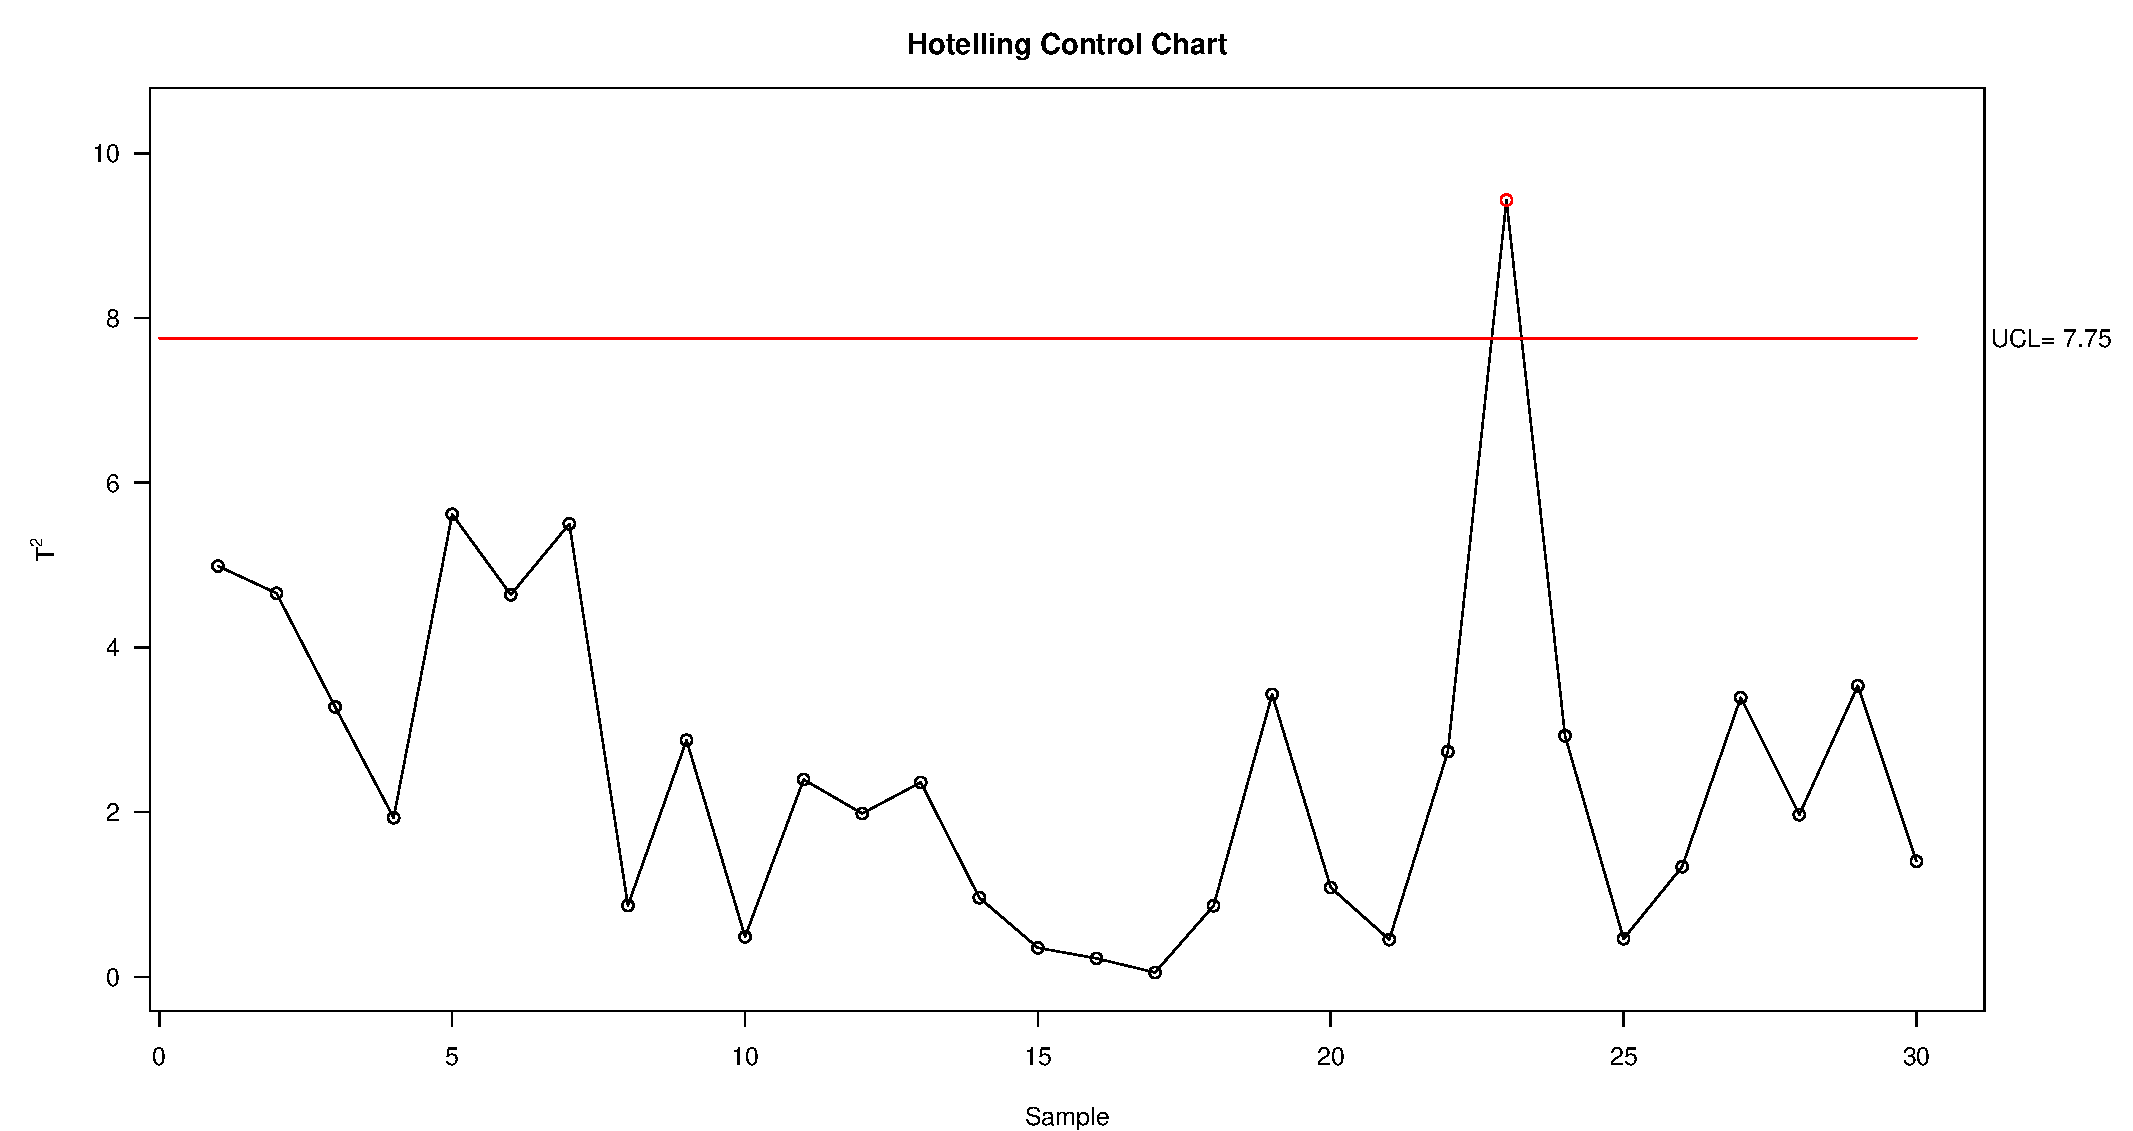
\includegraphics[scale=0.3]{FigurasUV/GT2.pdf}
  \caption{Ejemplo gráfico de control $T^2$ de Hotelling}
\end{figure}
\end{frame}

\begin{frame}{Gráfico de control de varianza generalizada}
De la misma manera que en el gráfico de control univariado, el monitor de la media del proceso está acoplado con un gráfico de dispersión; El seguimiento de la variabilidad del proceso resulta extremadamente útil en problemas multivariados. Esto se debe a que en el gráfico multivariado de Shewhart se asumió que la dispersión del proceso se mantuvo constante. Esta hipótesis debe comprobarse en la práctica.

~\\Hasta la fecha, se han propuesto varios métodos para el monitoreo simultáneo de la variabilidad, pero claramente el gráfico de varianza generalizada es el más aceptado. El término varianza generalizada se conoce como el determinante de la matriz de covarianza.

~\\Este tipo de gráfico resulta al trazar el determinante de la matriz de covarianza junto con los límites de control superior e inferior naturales. Cuando se conoce la matriz de covarianza S, los parámetros del gráfico dan como resultado
\begin{center}
$UCL=|\Sigma|(b_1 + 3b_2^{1/2})$

$CL=b_1|\Sigma|$

$LCL=max\left\lbrace|\Sigma|(b_1 -3b_2^{1/2}), 0\right\rbrace$
\end{center}
\end{frame}

\begin{frame}{Gráfico de control de varianza generalizada}
Donde
\begin{center}
$b_1=\frac{1}{(n-1)^p}\prod\limits_{j=1}^{p}(n-j)$

$b_2=\frac{1}{(n-1)^{2p}}\prod\limits_{j=1}^{p}(n-j)\left[\prod\limits_{i=1}^{p}(n-i+2)-\prod\limits_{i=1}^{p}(n-1)\right]$
\end{center}
Tenga en cuenta que n debe ser mayor que el número de características de calidad (p).

Con frecuencia, $\Sigma$ se desconoce y se estima a través de $\Sigma$ según la relación:
$$|S|=b_1|\Sigma|$$
Por lo tanto, los parámetros resultan en
\begin{center}
$UCL=\frac{S}{b_1}(b_1 + 3b_2^{1/2})$

$CL=|S|$

$LCL=max\left\lbrace\frac{|S|}{b_1}(b_1 -3b_2^{1/2}), 0\right\rbrace$
\end{center}

Teniendo en cuenta que S es una matriz positiva definida, el LCL carece de sentido para los valores negativos.
\end{frame}

\begin{frame}{Gráfico de control de varianza generalizada}
\begin{figure}[h!]
  \centering
  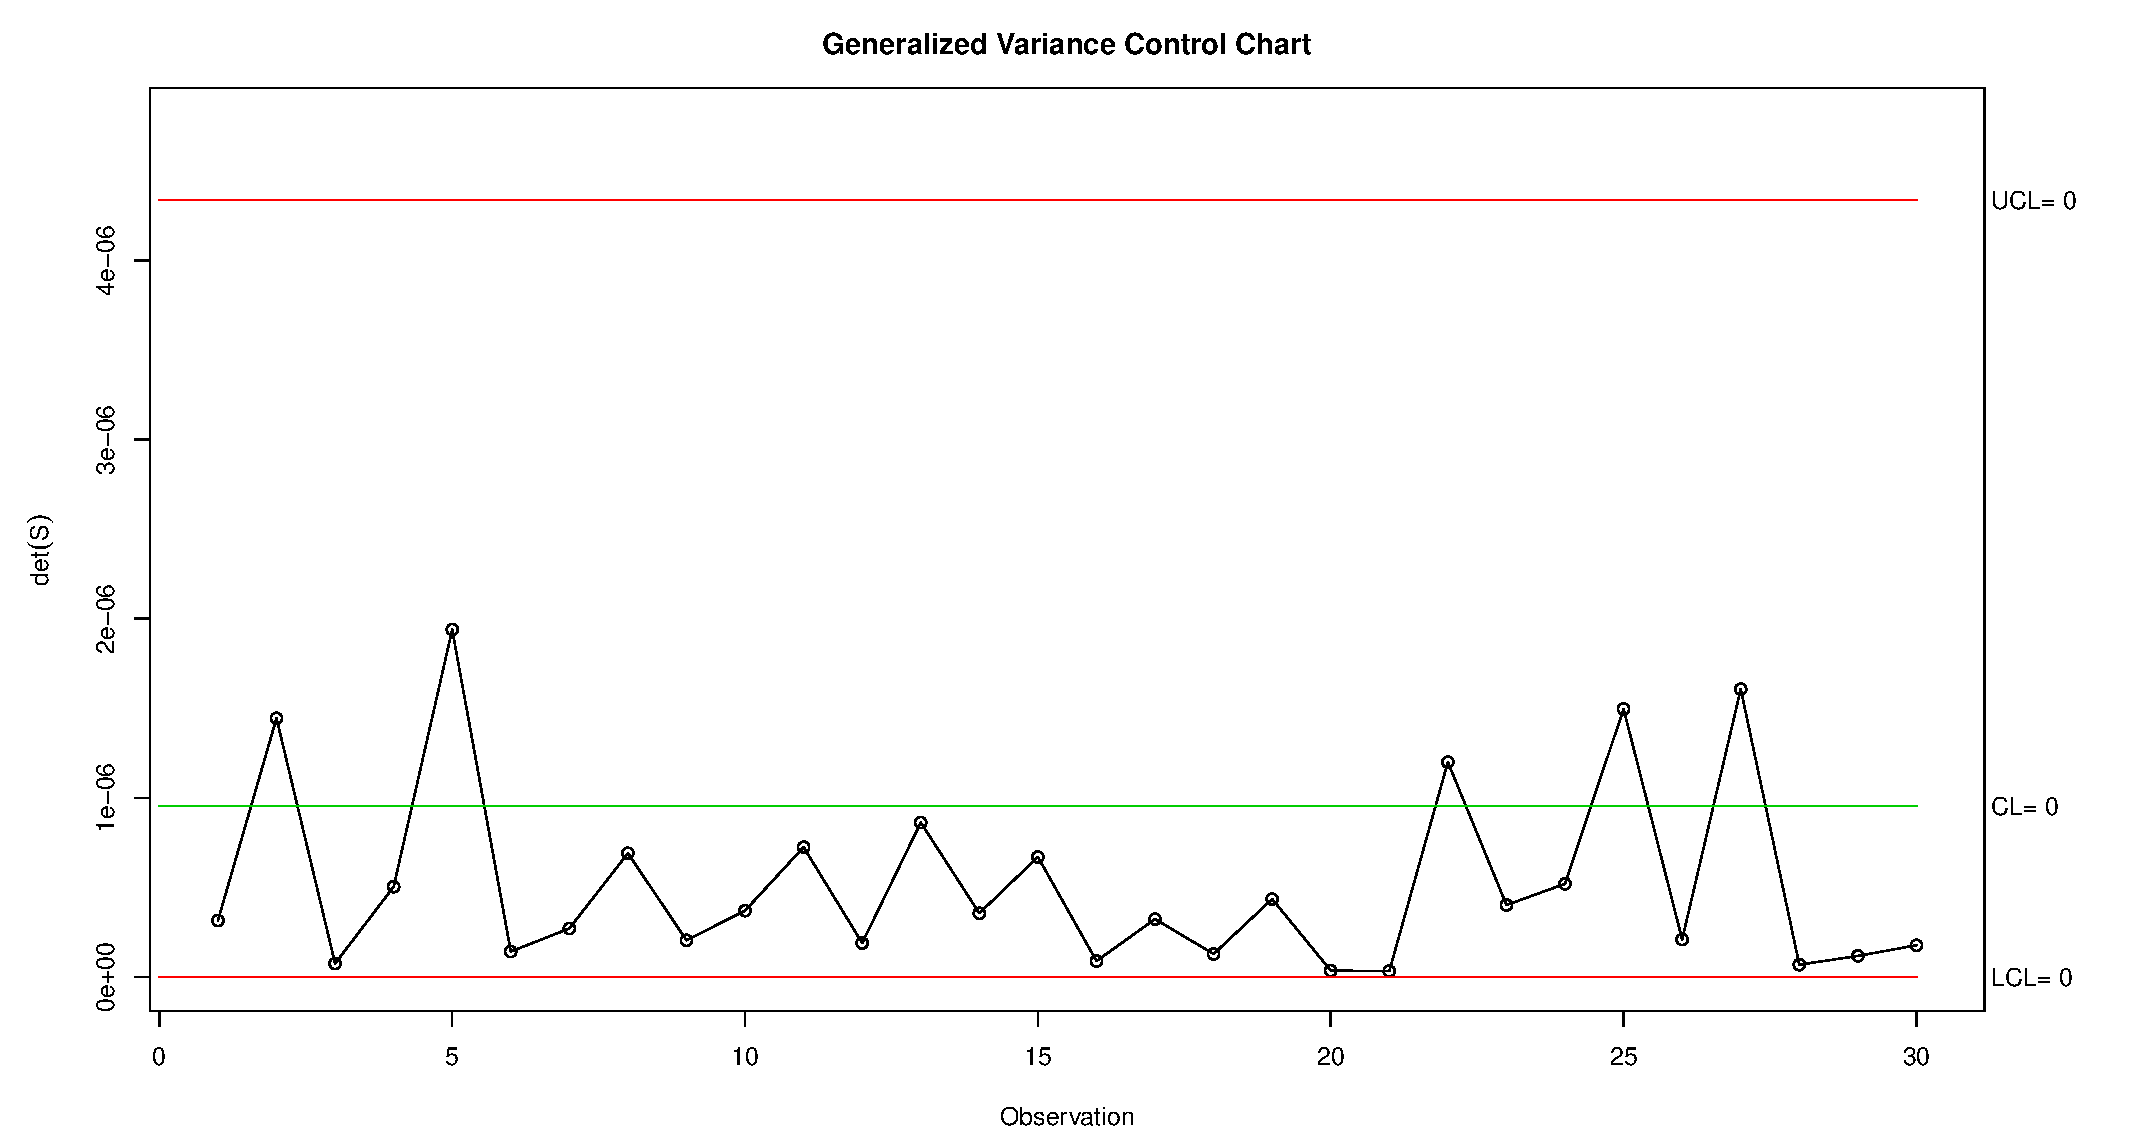
\includegraphics[scale=0.3]{FigurasUV/GVG.pdf}
  \caption{Ejemplo gráfico de control de varianza generalizada}
\end{figure}
\end{frame}

\begin{frame}{Gráfico multivariante de promedios ponderados exponencialmente MEWMA}
MEWMA es la extensión multivariable natural del gráfico EWMA propuesto por Roberts (1959). Fue introducido por Lowry et al. (1992) y es más sensible en la detección de cambios no aleatorios en el proceso y se basa en el principio del promedio ponderado de los vectores observados anteriormente. El gráfico MEWMA tiene las estadísticas:
$$T^2=Z'_i\Sigma_{Z_i}^{-1}Z_i >h$$
Donde
$$Z_i=\lambda X_i+(1-\lambda)X_{i-1}$$
Siendo $Z_0=0$,$\lambda$ es una matriz diagonal $p\;x\;p$ de constantes de suavizado con $0<\lambda_i\leq 1$, aunque en la práctica no hay razón para emplear valores diferentes de $\lambda$ en el mismo problema. En la práctica, el valor más utilizado de $\lambda$ es 0.1. En un caso particular, cuando se obtienen subgrupos racionales, es decir, $n > 1$, simplemente reemplace $X_i$ por $\bar{X}_i$.
\end{frame}

\begin{frame}{Gráfico multivariante de promedios ponderados exponencialmente MEWMA}
Lowry et al. (1992) proporcionan dos alternativas para calcular el tamaño, la matriz de covarianza exacta:
$$\Sigma_{Z_i}=\frac{\lambda\left[1-(1-\lambda)^{2i}\right]}{2-\lambda}(\Sigma)$$
Y, la llamada matriz de covarianza asintotica:
$$\Sigma_{Z_i}=\frac{\lambda}{2-\lambda}(\Sigma)$$
El primero teniendo un mejor desempeño.
Además, señalan que el rendimiento de ARL del gráfico depende solo del parámetro de no centralidad $\theta$:
$$\theta=\left[(\mu_1-\mu_0)'\Sigma (\mu_1-\mu_0)\right]^{1/2}$$
Donde $\mu_1$ es el vector de medias para la fase II. Note que cuando $\lambda=1$ el gráfico MEWMA es transformado en el gráfico $T^2$.
\end{frame}

\begin{frame}{Gráfico multivariante de promedios ponderados exponencialmente MEWMA}
\begin{figure}[h!]
  \centering
  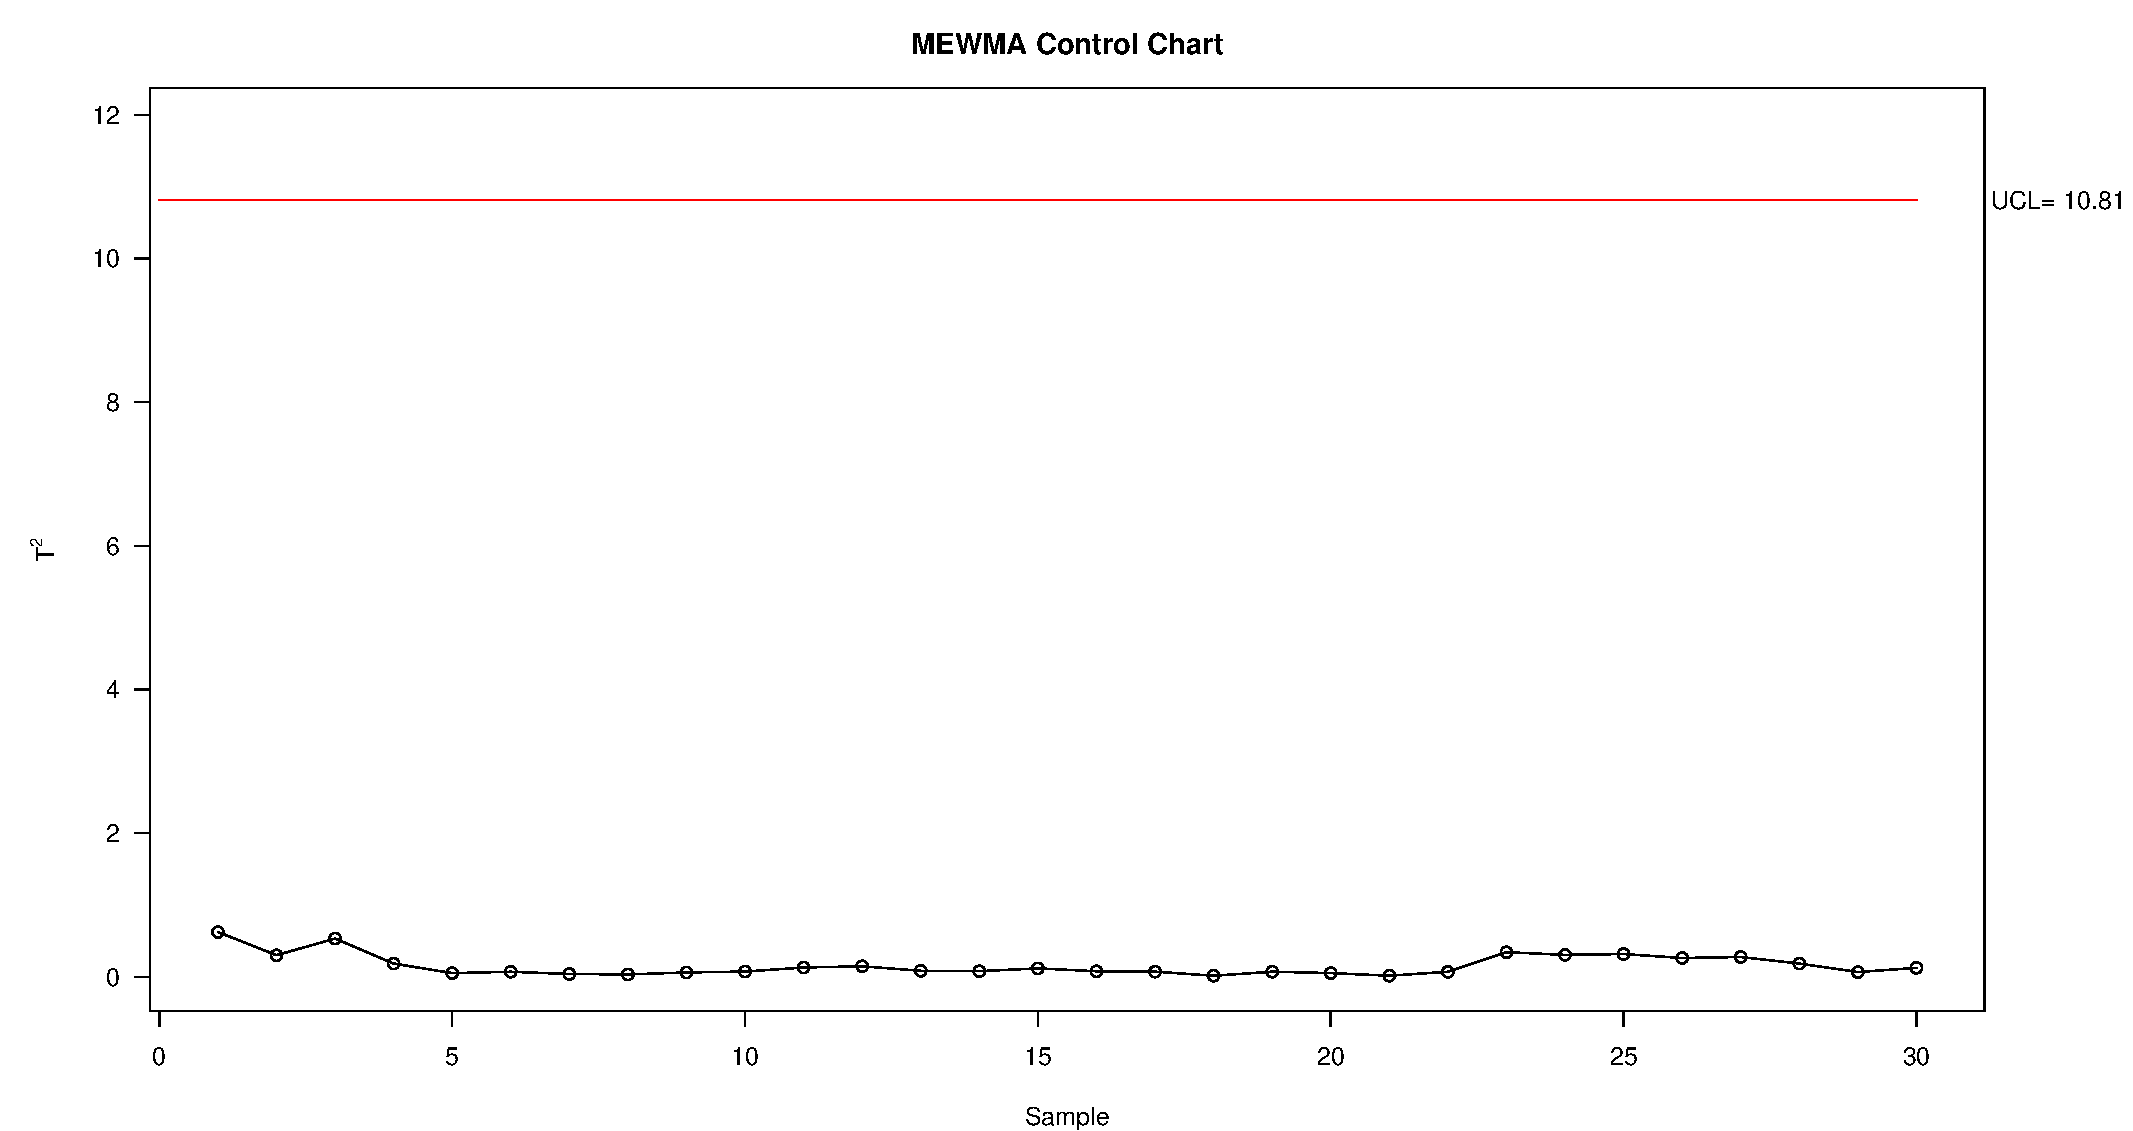
\includegraphics[scale=0.3]{FigurasUV/MEWMA.pdf}
  \caption{Ejemplo gráfico de control multivariante de promedios ponderados exponencialmente MEWMA}
\end{figure}
\end{frame}

\begin{frame}{Gráfico multivariante de suma acumulativa MCUSUM}
El gráfico de control MCUSUM aparece como la extensión multivariada del gráfico de control CUSUM propuesto originalmente por Page (1961). Se enfoca en mejorar la sensibilidad con respecto al gráfico $T^2$ previamente introducido al detectar pequeños cambios en el proceso y se basa en el principio de acumular información de las observaciones anteriores. Además del gráfico MEWMA, MCUSUM es un gráfico de la Fase II. Hay cuatro alternativas principales aceptadas para construir un gráfico MCUSUM, por limitaciones en la extensión nos enfocaremos en las dos propuestas que están implementadas en R, MCUSUM de acuerdo a Crosier (1988) y MCUSUM de Pignatiello y Runger (1990).
\end{frame}

\begin{frame}{MCUSUM Crosier (1988)}
Crosier (1988) presentó dos procedimientos multivariados. Se presenta la versión que tiene un mejor desempeño. El estadístico es:
$$T_i^2=\left[S'_i\left(\frac{\Sigma}{n}\right)^{-1}S_i\right]^{1/2}>h$$
Donde 
\begin{equation*}
S_i=\left\{
\begin{aligned}
0 \;\;\;\;\;\;\;\;\;\; si \;\;\; C_i\leq k\\
(S_{i-1}+\bar{X_{i}}-\mu_0)(1-\frac{k}{C_i}) \;\;\;\;\; si \;\;\; C_i> k
\end{aligned}
\right.
\end{equation*}
Donde $S_0=0,\; k>0$, y
$$C_i=\left[(S_{i-1}+\bar{X_{i}}-\mu_0)'\left(\frac{\Sigma}{n}\right)^{-1}(S_{i-1}+\bar{X_{i}}-\mu_0)\right]^{1/2}$$
Asimismo, el límite es
$$UCL=h$$
\end{frame}

\begin{frame}{MCUSUM Pignatiello y Runger (1990)}
Pignatiello y Runger también propusieron dos gráficos, el siguiente es el que tuvo mejor rendimiento:
\begin{equation*}
T_i^2=max\left\{
\begin{aligned}
0 \\
\left[S'_i\left(\frac{\Sigma}{n}\right)^{-1}S_i\right]^{1/2-kn_i}
\end{aligned}
\right.
\end{equation*}
Donde
$$S_i=\sum\limits_{j=1-n_i+1}^{i}(\bar{X_i}-\mu_0)$$
Y
\begin{equation*}
n_i=max\left\{
\begin{aligned}
n_{i-1}+1 \;\;\;\;\; si \;\;\;\;\;  T^2_{i-1}>0 \\
1 \;\;\;\;\; En\; otro\; caso
\end{aligned}
\right.
\end{equation*}
$$UCL=h$$
\end{frame}

\begin{frame}{Gráfico MCUSUM}
\begin{figure}[h!]
  \centering
  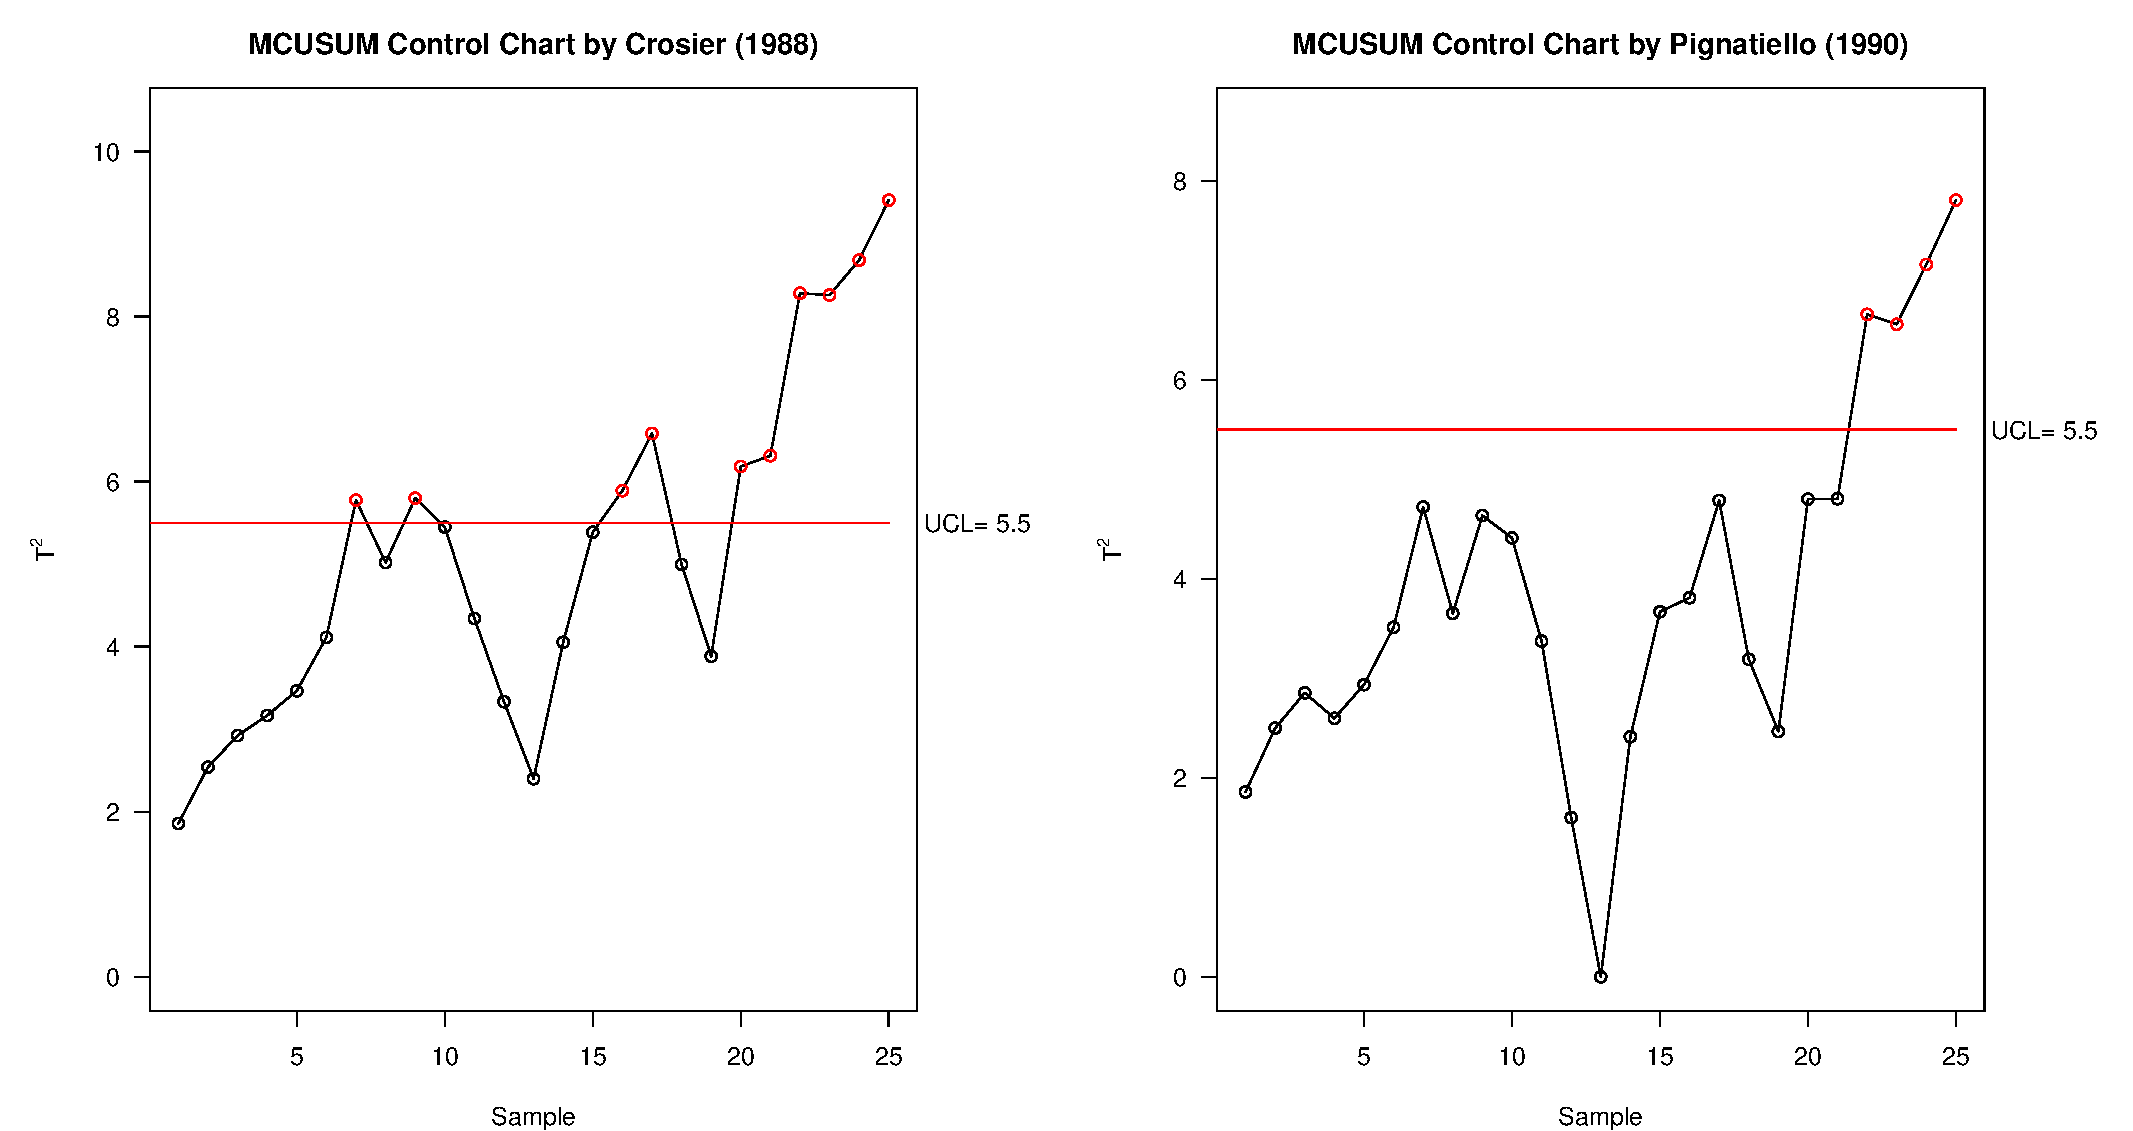
\includegraphics[scale=0.33]{FigurasUV/MCUSUM.pdf}
  \caption{Ejemplo gráficos de control MCUSUM}
\end{figure}
\end{frame}

\section{Caso ilustrativo: Control de Pitcheo}
\begin{frame}{Caso ilustrativo}
En este caso ilustrativo, la aplicación de los gráficos de control multivariados se introducen en el béisbol utilizando el software \cite{R}, específicamente sobre el desempeño del lanzador. Si bien los lanzadores mueven la pelota estratégicamente en diferentes posiciones de la zona de ataque intentando que el bateador no haga contacto con ella, a menudo el desempeño del lanzador se mide por la habilidad para poner la bola en la zona de golpe a alta velocidad.

~\\En este caso, utilizamos los datos recopilados por los registros de lanzadores en la base de datos (MLB) para el lanzador C.C. Sabathia de los New York Yankees. Se seleccionaron dos conjuntos de datos de los juegos contra Tampa Bay: el primero el 10 de julio de 2011 y el 12 de agosto de 2011 el segundo. Ambos se almacenan en el paquete \cite{R1} como sabathia1 y sabathia2 respectivamente. Los registros del lanzador brindan mucha información sobre cada lanzamiento, pero en nuestro estudio trabajamos con la velocidad de inicio (dada en mph) del lanzamiento y la ubicación (en pies) cuando cruza la casa. Solo se consideran los lanzamientos de bola rápida y cada muestra es un bateador promediando todas las variables de lanzamiento. Observa que un jugador bate varias veces en la jugada.
\end{frame}

\begin{frame}{Caso ilustrativo}
El vector de medias, la matriz de varianzas y covarianzas y la matriz de correlaciones son:
\begin{equation*} 
\bar{x}=\begin{bmatrix} 
0.1069565   \\ 
 2.9430435  \\
 94.4108696  
\end{bmatrix} \; ; \; 
S=\begin{bmatrix} 
0.22087668 & 0.09182787 & 0.05130731\\
0.09182787 & 0.27479486 &-0.25359822\\
0.05130731 & -0.25359822& 1.50752648
\end{bmatrix}
\end{equation*}
\begin{equation*}
r=\begin{bmatrix}
1.00000000 & 0.3727308 & 0.08891435 \\
0.37273078 & 1.0000000 &-0.39401198 \\
0.08891435 & -0.3940120&  1.00000000 \\
\end{bmatrix}
\end{equation*}

~\\Se puede realizar un análisis útil inicial mediante la construcción de un diagrama de dispersión tridimensional con un elipsoide de confianza.
\end{frame}

\begin{frame}{Caso ilustrativo}
\begin{figure}[h!]
  \centering
  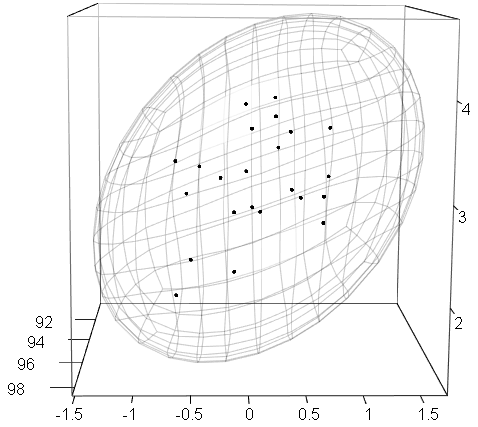
\includegraphics[scale=0.45]{FigurasUV/ELIPSE.png}
  \caption{Diagrama de dispersión tridimensional con confianza elipsoide}
\end{figure}
Al moverse a través de las coordenadas, se puede ver que todas las observaciones caen dentro de estos límites. No se detectan valores atípicos. 
\end{frame}

\begin{frame}{Caso ilustrativo}
Al realizar un gráfico de Hotelling, obtenemos
\begin{figure}[h!]
  \centering
  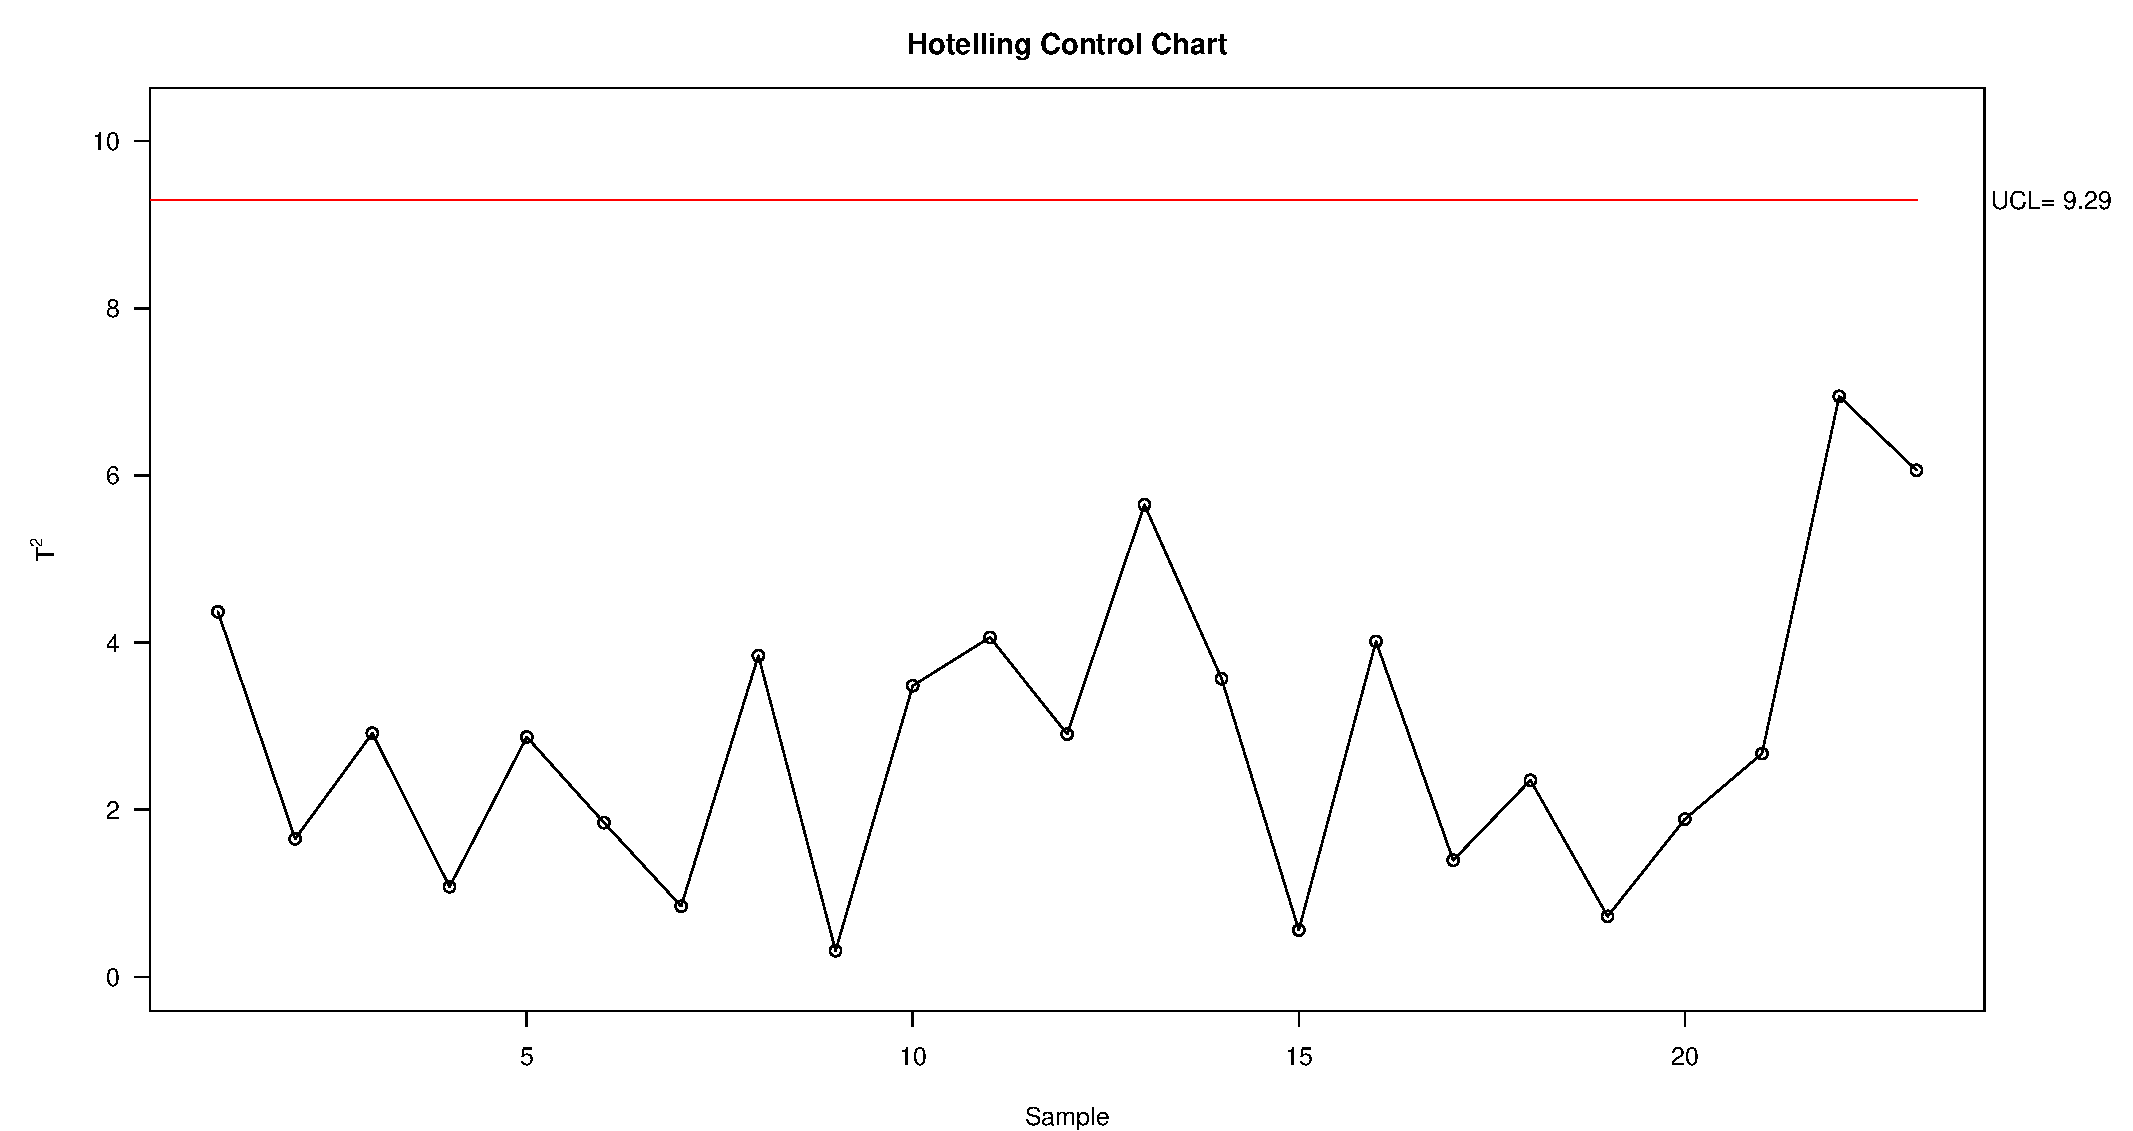
\includegraphics[scale=0.26]{FigurasUV/HTS1.pdf}
  \caption{Gráfico de control $T^2$ de Hotelling para los datos de sabathia 1}
\end{figure}
Dado que no hay puntos fuera del UCL, no hay evidencia para rechazar el estado de control en el proceso. 
\end{frame}

\begin{frame}{Caso ilustrativo}
Luego, Se utiliza este primer juego para analizar el segundo juego como Fase II u observaciones futuras, utilizando las estimaciones de Fase I del vector medio y la matriz de covarianza.
\begin{figure}[h!]
  \centering
  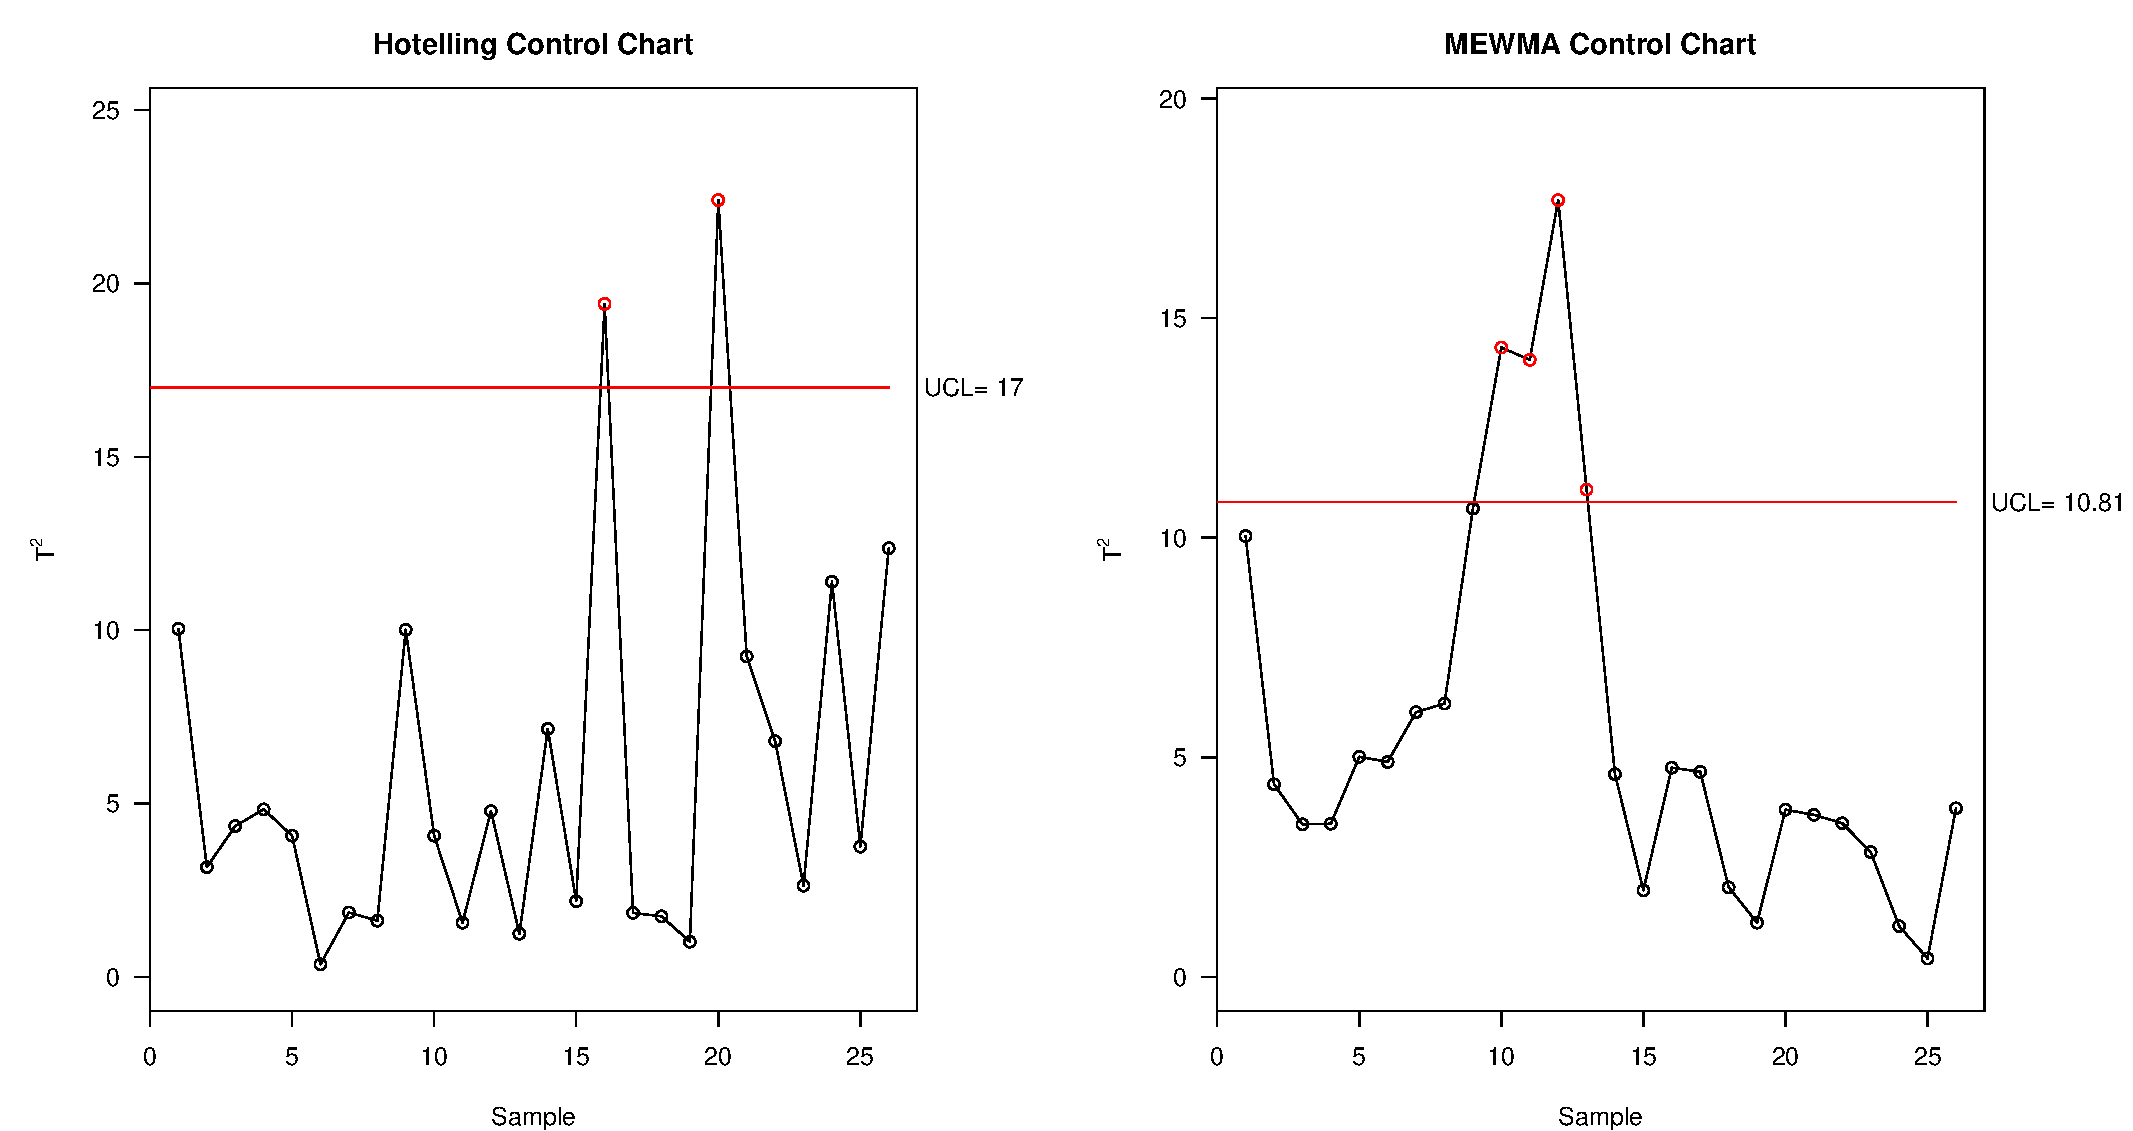
\includegraphics[scale=0.3]{FigurasUV/HMS2.pdf}
  \caption{Gráficos de control $T^2$ de Hotelling y MEWMA para los datos sabathia2}
\end{figure}
\end{frame}

\begin{frame}{Caso ilustrativo}
Para detectar cuál o cuáles variables originaron que el proceso se saliera de control, y poder corregir el problema, se utiliza un proceso denominado descomposición del estadístico $T^2$, la cual obtiene el estadístico $T^2$ y el $UCL$ con cada una de las variables individuales, luego con pares de variables para las posibles combinaciones y finalmente para las 3 variables. La variable o variables para las cuales el $T^2$ calculado supera el valor del $UCL$ calculado son las que originaron que el proceso se saliera de control. 
\begin{figure}[h!]
  \centering
  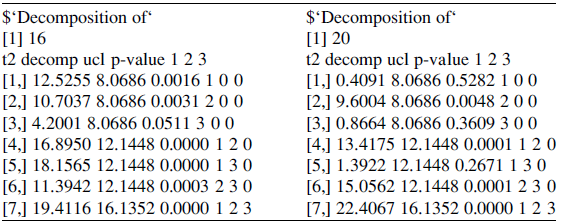
\includegraphics[scale=0.6]{FigurasUV/DescT2.png}
  \caption{Descomposición estadístico $T^2$ para detectar variables fuera de control}
\end{figure}
\end{frame}

\begin{frame}{Caso ilustrativo}
\begin{figure}[h!]
  \centering
  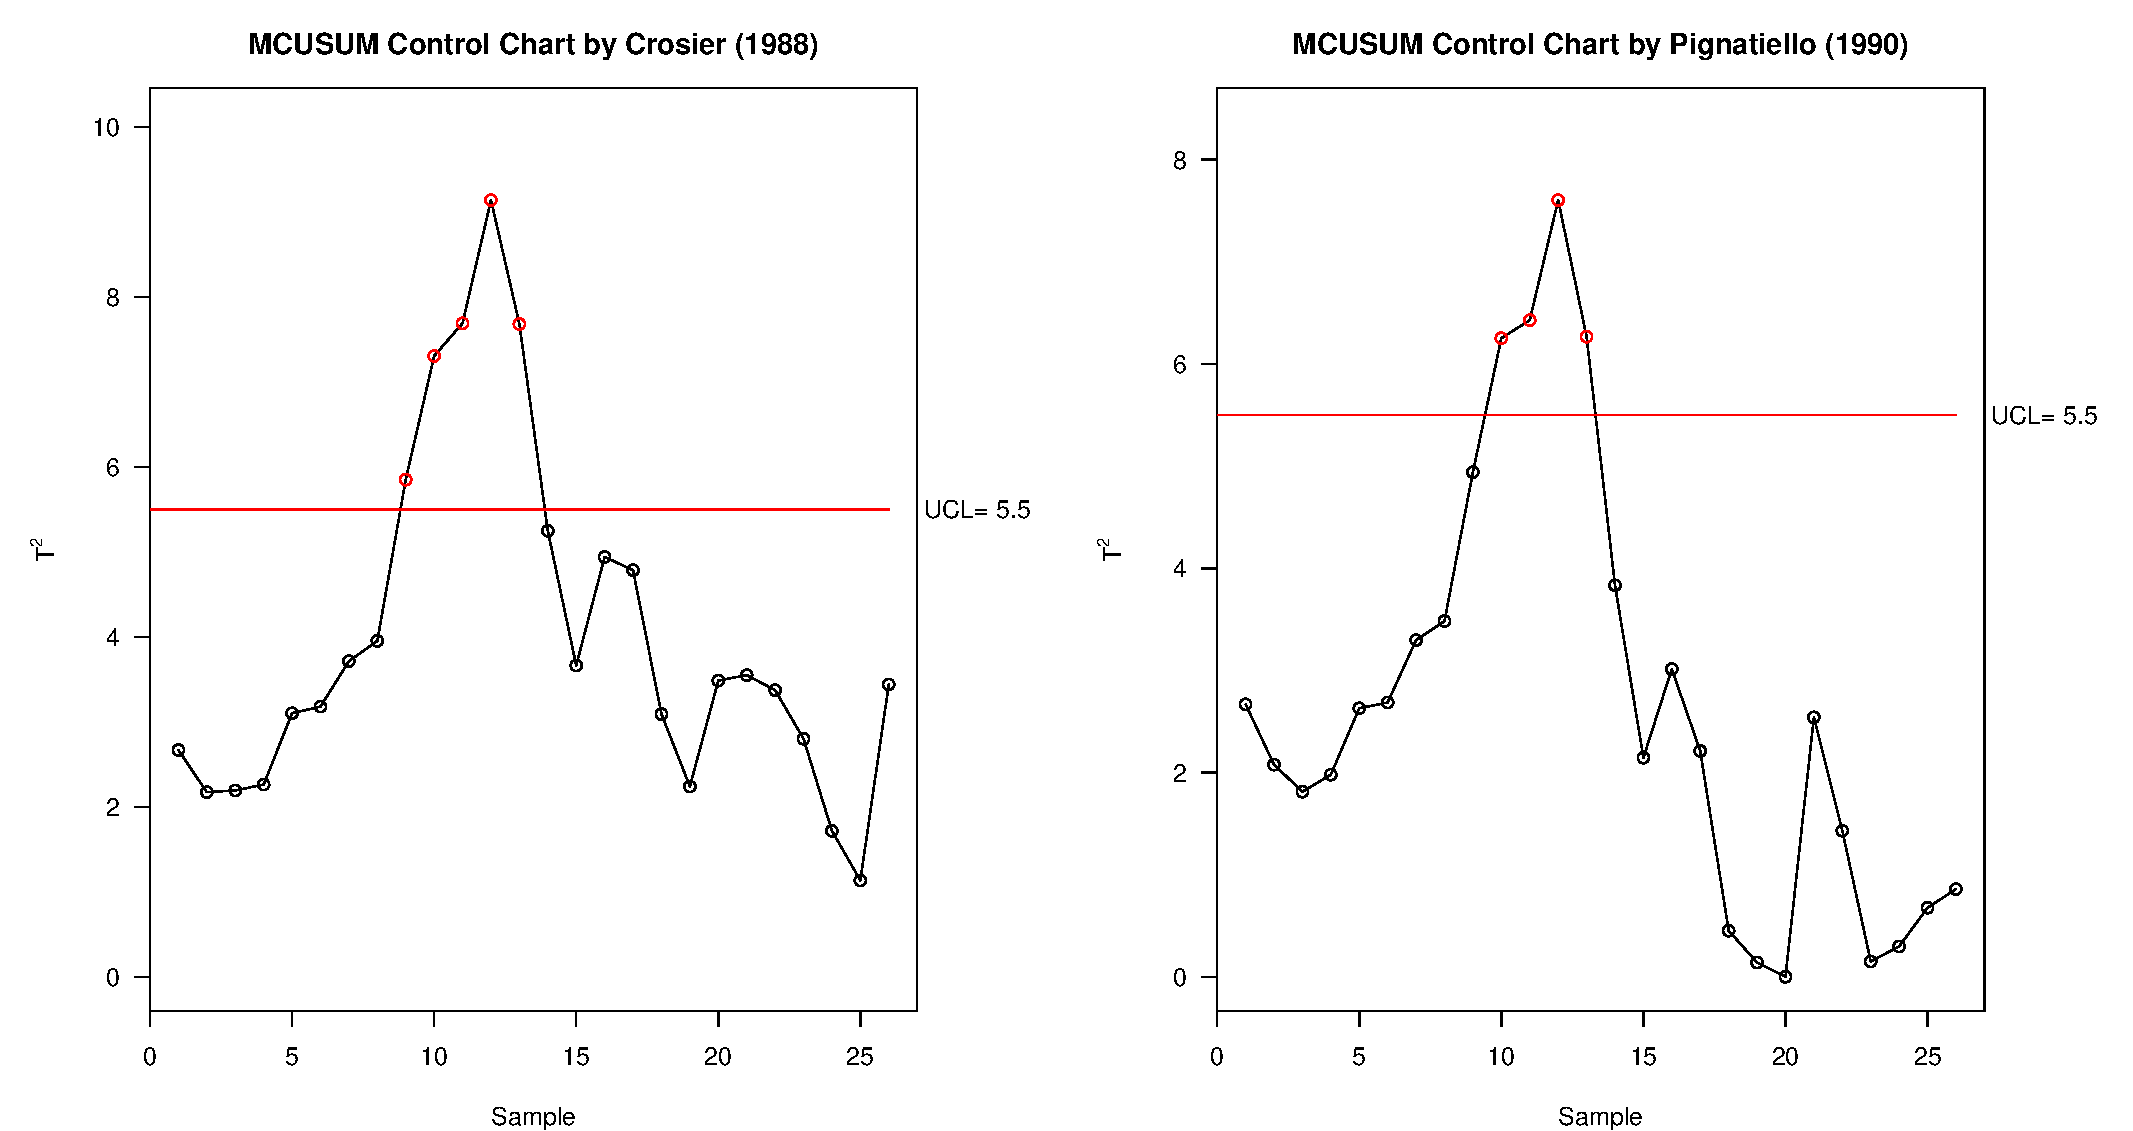
\includegraphics[scale=0.27]{FigurasUV/MC1y2.pdf}
  \caption{Gráfico de control CUSUM por Crosier 1988 y Pignatiello 1990 para los datos de sabathia2}
\end{figure}

El MCUSUM según (Crosier 1988) y (Pignatiello y Runger 1990) detectaron cambios en la media en los 9º y 10º bateadores respectivamente.
\end{frame}

\section{Conclusiones}
\begin{frame}{Conclusiones}
Como conclusión general se tiene que los gráficos de control multivariantes son una herramienta muy útil y muy potente en el control estadístico de la calidad, permitiéndonos detectar cuando un proceso se sale de control con una alta precisión. Dentro de los gráficos mencionados, se vio que el gráfico de control $T^2$ de Hotelling tiene un buen desempeño en la detección de grandes cambios en la media, sin embargo, se queda corto ante cambios pequeños que presente el proceso; por ello se utilizan también los gráficos MEWMA y MCUSUM los cuales mejorar la detección rápida de pequeños cambios en el proceso, en el ejemplo aplicado se vio que estos últimos detectaban más rápido los cambios en el desempeño de los lanzamientos del jugador. 
\nocite{LGCM,LGCM1}
\end{frame}


\bibliographystyle{plain}
\bibliography{references}
\end{document}
